\documentclass{template}

% Set the background image
\setBackground{docs/img/background2.png}

\begin{document}

% Title Page
\begin{titlepage}
    \centering
    \vspace*{0.5in}
    {\Huge \textbf{Nexus : Les échos de la chute}}\\

    \vspace{0.5in}
    \addLogoWithGradient[1]{docs/img/logo.png}\\[1cm]
    \vspace{0.5in}
    {\Large Une expérience immersive pour les passionnés d'airsoft}
    {\large \url{https://leroilion.github.io/airsoft---nexus-les-echos-de-la-chute}}
\end{titlepage}
% \newpage

% Content
\section{Introduction}

\textbf{La chute fut brutale...} \\ \\
Suite à la mutinerie à bord du Nova Prime, votre groupe a pu atteindre une capsule de survie in extremis. Vous vous réveillez dans un environnement à la fois hostile et mystérieux, entourés par une forêt dense et des montagnes imposantes qui se dressent à l'horizon.
\\ \\
En utilisant les scanners encore fonctionnels de votre capsule, la vérité se révèle progressivement :
\begin{itemize}
    \item Le reste de l'équipage, contre lequel vous vous étiez opposés, a lui aussi survécu et a atterri sur cette planète dans une autre capsule de survie.
    \item Le seul espoir de quitter cet enfer repose sur le téléporteur embarqué à bord de votre vaisseau, désormais écrasé et endommagé.
    \item Les circuits de programmation n'étant plus en place, il vous faut les récupérer pour réactiver cet appareil essentiel.
\end{itemize}
Une course contre la montre s'engage. Votre mission est claire : trouver les circuits manquants, les programmer et activer le téléporteur avant que l'autre faction de l'équipage ne vous abandonne ici, voués à une mort certaine sur cette planète inhospitalière.\\
\\
Que votre stratégie et votre esprit d'équipe vous mènent à la victoire... ou à la survie.


\section{Déroulement de la partie}

Chaque équipe a pour mission de récupérer des cartes nécessaires à la programmation du téléporteur. Une fois trouvées, ces cartes doivent être programmées aux couleurs de l'équipe avant d'être insérées dans le téléporteur central. La coordination et la stratégie seront cruciales pour surmonter les obstacles adverses et atteindre cet objectif.

\section{Fin de la partie}

La partie prend fin dans l'un des cas suivants :
\begin{itemize}
    \item Lorsque le téléporteur est définitivement détruit, le temps imparti étant écoulé.
    \item Lorsque plus de la moitié des cartes insérées dans le téléporteur appartiennent à une même équipe, marquant leur victoire.
\end{itemize}

\section{Zone de jeu}

L'intégralité du terrain d'airsoft est utilisée pour ce scénario. Le téléporteur est positionné au centre, servant de point stratégique majeur.


\begin{itemize}
    \item Dans la variante \textit{Rivalité programmée}, un programmateur sera également placé sur le terrain, entre les zones de départ des deux équipes.
    \item Dans les variantes \textit{Course aux fragments} et \textit{Rivalité programmée}, des cartes seront dispersées aléatoirement à travers le terrain, renforçant l'importance de l'exploration et du contrôle des zones.
\end{itemize}

\section{Eléments de jeu}

Les éléments nécessaires au bon déroulement du scénario sont les suivants :

\begin{itemize}
    \item \textbf{Le téléporteur central :} point stratégique principal (description détaillée en annexe).
    \item \textbf{Les cartes de programmation :} indispensables pour activer le téléporteur (description détaillée en annexe).
    \item \textbf{Les lecteurs portables et les programmateurs de cartes :} outils permettant de scanner et programmer les cartes (description détaillée en annexe).
\end{itemize}

\section{Variantes}

Avant d’aborder les spécificités de chaque variante, voici les règles communes à respecter pour garantir une expérience de jeu équilibrée et immersive :

\subsection*{Règles du jeu}

\begin{enumerate}
    \item \textbf{Cartes insérées :} Une fois une carte insérée dans le téléporteur, elle ne peut plus être retirée sous aucun prétexte.
    \item \textbf{Lancé interdit :} Il est strictement interdit de lancer un élément de jeu, que ce soit une carte, un accessoire ou tout autre objet. Cette règle vise à protéger le matériel et à garantir la sécurité de tous les participants.
    \item \textbf{Joueur touché :} Si vous êtes touché, deux options s'offrent à vous :
    \begin{itemize}
        \item \textbf{Soins sur le terrain :} Trouvez un camarade médecin pour soigner vos blessures pendant \textbf{10 secondes}. Cependant, chaque joueur ne peut être soigné sur le terrain \textbf{qu'une seule fois} par cycle de respawn. 
        \item \textbf{Retour au respawn :} endez-vous à votre point de respawn et attendez \textbf{30 secondes} avant de revenir en jeu. Une fois revenu, vous redevenez éligible à un soin sur le terrain.
    \end{itemize}
    \item \textbf{Restrictions pour les médecins :}
    \begin{itemize}
        \item Si un médecin est touché pendant un soin, il doit immédiatement se déclarer "OUT", et le blessé reste sans soins.
        \item Pendant un soin, un médecin ne peut utiliser aucune arme.
        \item Le médecin doit poser ses deux mains sur le blessé pour le soigner et lui permettre de reprendre le combat.
        \item Si nécessaire, le médecin peut déplacer le blessé d’un pas pour le mettre à l’abri.
    \end{itemize}
    \item \textbf{Annonce des statuts :}
    \begin{itemize}
        \item Lorsqu'un joueur est touché, il doit le signaler en criant \textbf{"OUT"} de manière claire et audible.
        \item Lorsqu'un joueur reprend le jeu après un soin ou un respawn, il doit annoncer \textbf{"REPRISE"}. 
    \end{itemize}
    \item \textbf{Fin de partie :} Avant de quitter le terrain, effectuez un tour rapide des zones où vous avez laissé tomber des cartes afin d’aider les organisateurs à récupérer tous les éléments de jeu.
    \item \textbf{Fairplay :} Le fairplay est une valeur fondamentale de toute partie d'airsoft. Chaque joueur est tenu de respecter les règles et ses adversaires pour garantir une expérience agréable et équitable.
\end{enumerate}

\subsection{Transport à Haut Risque}  % Chaque équipe part avec les cartes déjà dans son camp, mais ne peux les transporter qu'une par une jusqu'au téléporteur

\begin{minipage}[t]{0.48\textwidth}
    \vspace{0em}
    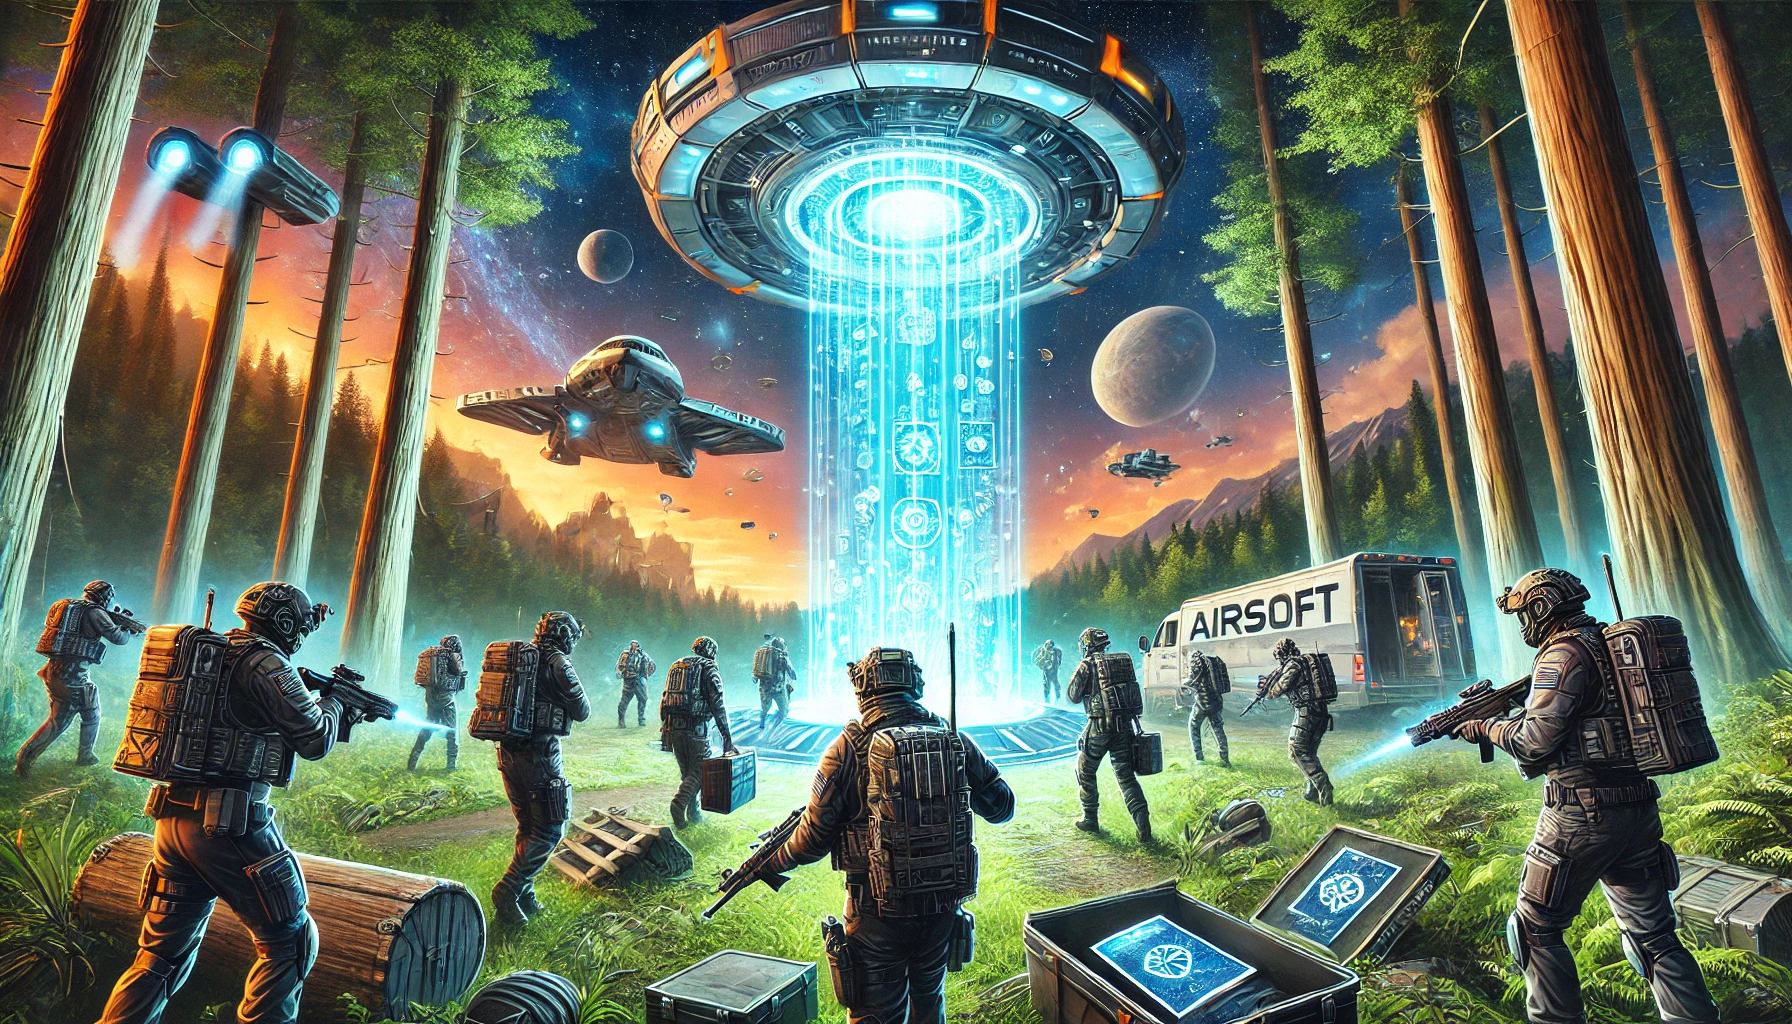
\includegraphics[width=\linewidth]{docs/img/variante1.png}
\end{minipage}
\hfill
\begin{minipage}[t]{0.48\textwidth}
    Dans votre malheur, vous bénéficiez d’une chance inespérée : les 5 cartes nécessaires pour réparer le téléporteur sont déjà en votre possession, sécurisées dans votre capsule de survie. Cependant, elles sont extrêmement instables : les transporter ensemble risque de les déprogrammer. Vous devez donc les acheminer une par une jusqu’au téléporteur central, en évitant toute erreur ou embuscade.
\end{minipage}

\subsection*{Règles du jeu}

\begin{enumerate}
    \item \textbf{Transport limité :} Chaque équipe ne peut transporter qu’une seule carte à la fois. Une nouvelle carte ne peut être prise qu’après avoir inséré la précédente dans le téléporteur.
    \item \textbf{Cartes attribuées :} Les cartes sont attribuées à une équipe spécifique. Vous n’êtes pas autorisés à manipuler ou interférer avec les cartes de l’équipe adverse.
    \item \textbf{En cas d’élimination :} Si vous êtes éliminé et devez vous rendre au point de respawn, vous devez immédiatement déposer la carte transportée sur le sol à l’endroit où vous avez été touché. 
\end{enumerate}

Coordination et communication au sein de votre équipe seront essentielles pour éviter les pertes inutiles et optimiser votre progression. Ne perdez pas de temps, car chaque instant compte dans cette course contre la montre !

\subsection{Course aux Fragments}  % Les équipes doivent trouver les cartes sur le terrain et le programmer à leur couleur dans leur camp

\begin{minipage}[t]{0.48\textwidth}
    Malheureusement, les cartes nécessaires à la réparation du téléporteur se sont dispersées à travers la planète lors du crash. Votre mission : les retrouver, les rapporter jusqu’à votre capsule de sauvetage pour les programmer aux couleurs de votre équipe, puis les acheminer jusqu’au téléporteur. Mais méfiez-vous, l’ennemi pourrait bien essayer de vous voler vos trouvailles...
\end{minipage}
\hfill
\begin{minipage}[t]{0.48\textwidth}
    \vspace{0em}
    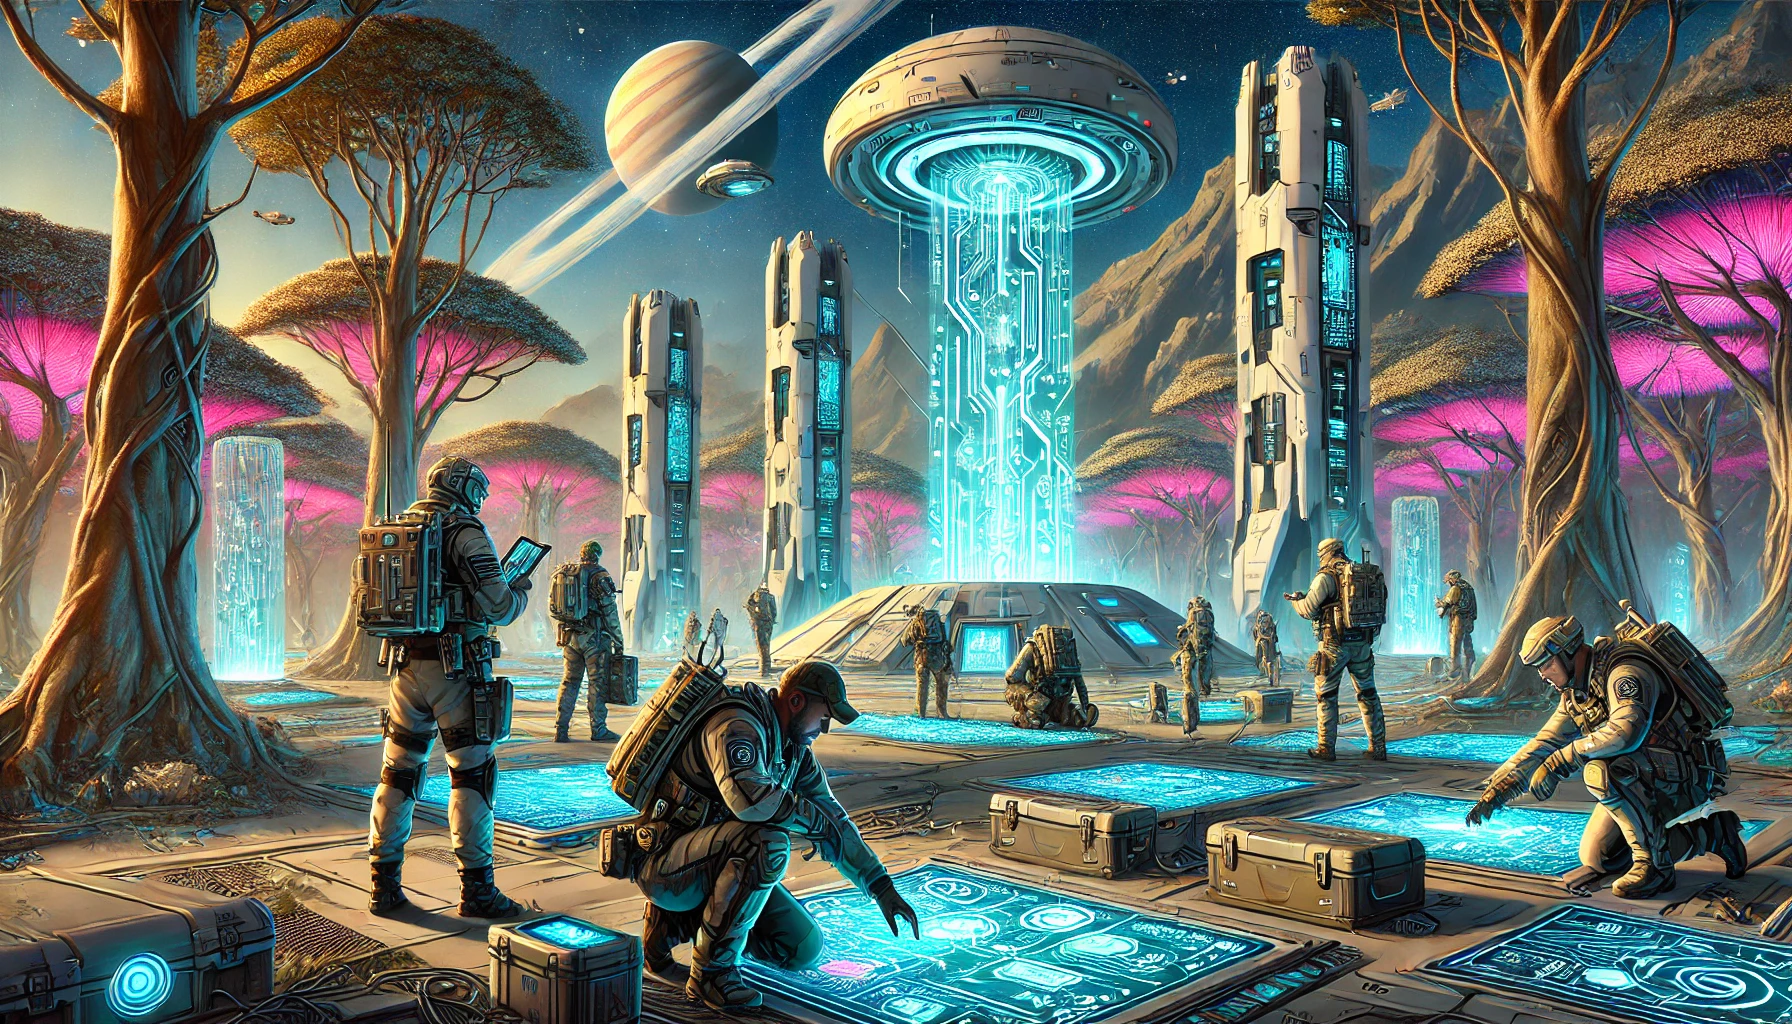
\includegraphics[width=\linewidth]{docs/img/variante2.png}
\end{minipage}

\subsection*{Règles du jeu}

\begin{enumerate}
    \item \textbf{Transport multiple :} Vous pouvez transporter plusieurs cartes par équipe, mais une seule par joueur. Restez vigilants face aux risques d’attaque, car chaque carte transportée augmente l’importance de votre sécurité.
    \item \textbf{En cas de joueur touché :}
    \begin{itemize}
        \item Retournez au point de respawn en laissant la ou la carte à l’endroit où vous avez été touché.\newline
        \textbf{OU}
        \item Restez sur place en attendant l’intervention d’un médecin. Cependant, si un joueur adverse ou allié vous demande une carte que vous transportez, vous êtes tenu de la lui remettre.
    \end{itemize}
\end{enumerate}

La rapidité est de mise, mais attention à ne pas aller trop vite et oublier un passage par le programmateur. il serait dommage de donner des points à l'adversaire ...

\subsection{Rivalité Programmée}  % Les équipes doivent trouver les cartes sur le terrain et le programmer à leur couleur avec le programmateur quelque part sur le terrain (accessible à toutes les équipes)

\begin{minipage}[t]{0.48\textwidth}
    \vspace{0em}
    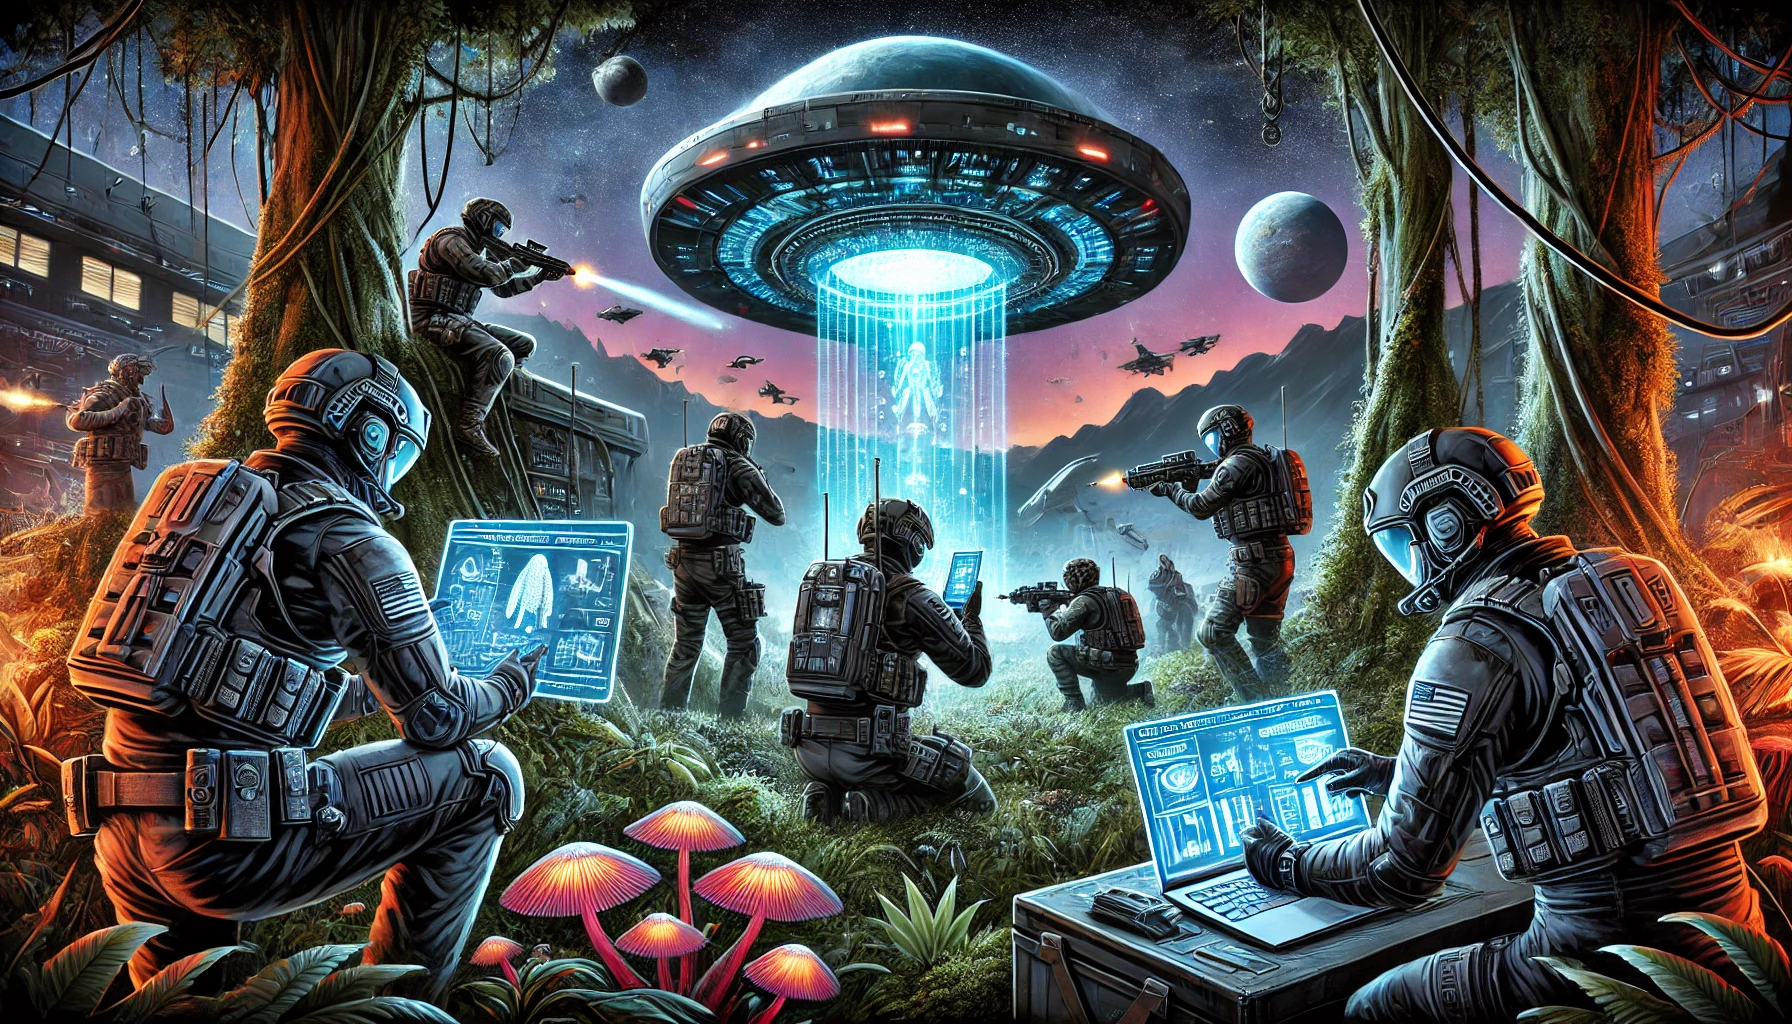
\includegraphics[width=\linewidth]{docs/img/variante3.png}
\end{minipage}
\hfill
\begin{minipage}[t]{0.48\textwidth}
Lors du scan de la planète, vous découvrez que les circuits dispersés à travers la planète ne sont pas correctement programmés. Malheureusement, l'ordinateur de votre capsule de survie, qui aurait pu les reprogrammer, est hors service. \\

Votre seule option : retrouver un fragment fonctionnel de l’ordinateur du vaisseau crashé et l’utiliser pour reprogrammer les circuits avant de les insérer dans le téléporteur central. 
\end{minipage}


\subsection*{Règles du jeu}

\begin{enumerate}
    \item \textbf{Transport multiple :} Vous pouvez transporter plusieurs cartes par équipe, mais une seule par joueur. Restez vigilants face aux risques d’attaque, car chaque carte transportée augmente l’importance de votre sécurité.
    \item \textbf{Ordinateur fixe :} L’ordinateur utilisé pour reprogrammer les circuits est un point fixe sur le terrain et ne peut pas être déplacé.
    \item \textbf{En cas de joueur touché :}
    \begin{itemize}
        \item Retournez au point de respawn en laissant la carte à l’endroit où vous avez été touché.\newline
        \textbf{OU}
        \item Restez sur place en attendant l’intervention d’un médecin. Cependant, si un joueur adverse ou allié vous demande une carte que vous transportez, vous êtes tenu de la lui remettre.
    \end{itemize}
\end{enumerate}

Allez-vous partir à la recherche des circuits perdus, défendre le téléporteur ou concentrer vos efforts pour protéger l’ordinateur de reprogrammation ? À vous de choisir la meilleure stratégie pour garantir votre survie et celle de votre équipe !

\subsection{La Course des Scientifiques}  % Les équipes doivent trouver les cartes sur le terrain et le programmer à leur couleur avec le programmateur des scientifiques

\begin{minipage}[t]{0.48\textwidth}
    Lors du crash, les cartes nécessaires à la réparation du téléporteur se sont déprogrammées et dispersées à travers la planète. Heureusement, un scientifique de votre équipe est équipé du matériel nécessaire pour reprogrammer ces cartes vitales. \\
    
    Votre mission est double : retrouver les cartes et les reprogrammer tout en assurant la protection du scientifique. Si ce dernier est blessé, il sera dans l’incapacité de reprogrammer les cartes, mettant ainsi votre équipe en difficulté. Une fois les cartes prêtes, il faudra les acheminer jusqu’au téléporteur central pour activer l’appareil.
\end{minipage}
\hfill
\begin{minipage}[t]{0.48\textwidth}
    \vspace{0em}
    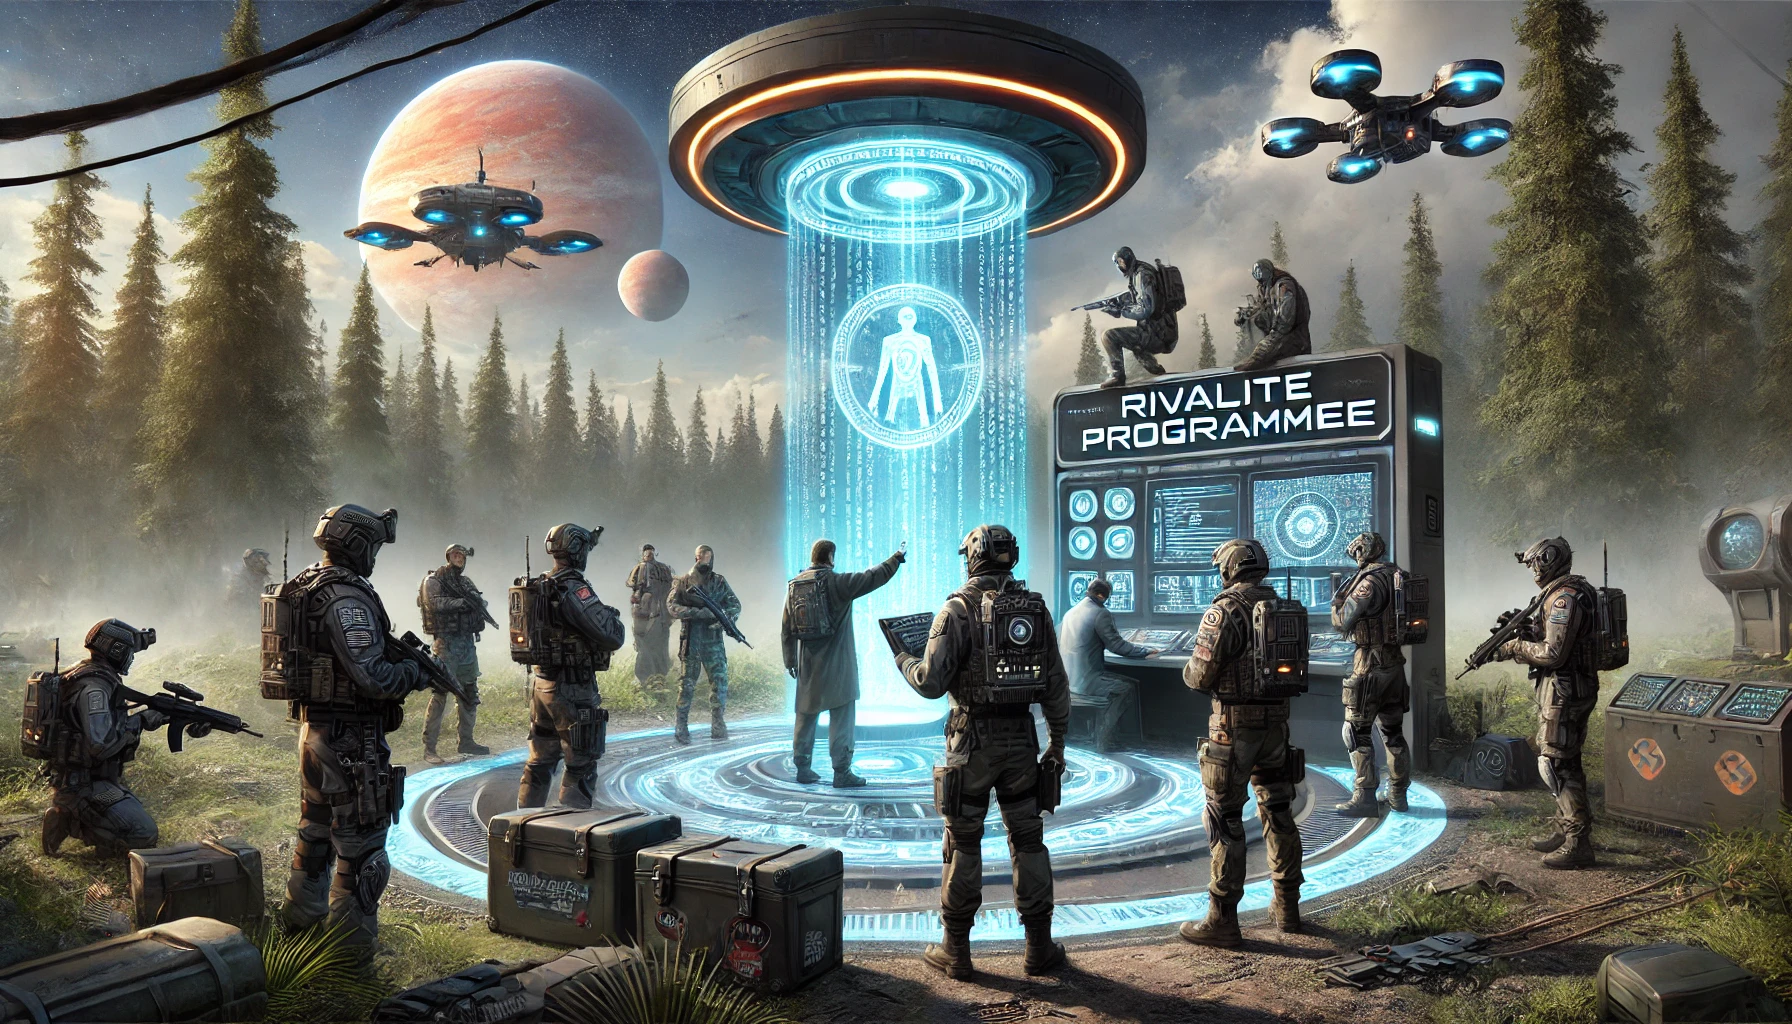
\includegraphics[width=\linewidth]{docs/img/variante4.png}
\end{minipage}


\subsection*{Règles du jeu}

\begin{enumerate}
    \item \textbf{Transport multiple :} Vous pouvez transporter plusieurs cartes par équipe, mais une seule par joueur. Restez vigilants face aux risques d’attaque, car chaque carte transportée augmente l’importance de votre sécurité.
    \item \textbf{Un seul scientifique :} Un joueur doit être désigné comme scientifique. Il sera le seul à pouvoir utiliser l’appareil de reprogrammation pour rendre les cartes utilisables par votre équipe.
    \item \textbf{Scientifique blessé :} Si le scientifique est touché, il ne pourra plus reprogrammer de cartes tant qu’il n’aura pas été soigné ou qu’il ne sera pas revenu du respawn.
    \item \textbf{En cas de joueur touché :}
    \begin{itemize}
        \item Retournez au point de respawn en laissant la carte à l’endroit où vous avez été touché.\newline
        \textbf{OU}
        \item Restez sur place en attendant l’intervention d’un médecin. Cependant, si un joueur adverse ou allié vous demande une carte que vous transportez, vous êtes tenu de la lui remettre.
    \end{itemize}
\end{enumerate}

Quelle stratégie adopterez-vous ? Positionner votre équipe en embuscade pour intercepter l’adversaire, quitte à exposer votre scientifique ? Ou concentrer vos efforts sur la récupération rapide des cartes et leur reprogrammation ? Chaque choix peut faire la différence entre la victoire et la défaite.






\section{Annexes}

Vous trouver sur mon dépot github tous les plans pour la fabrication des éléments de jeu.

\begin{itemize}
    \item \textbf{Les cartes} : 
    \item \textbf{Les lecteurs et programmateur} : 
    \item \textbf{Le téléporteur} : 
\end{itemize}


\end{document}
